\section{Own Experiment: Does Instruction Tuning Alone Cause Hyper-Accuracy?}
\label{sec:experiment}

Aher et al.\ link the hyper-accuracy distortion to alignment, but they could only compare API models whose training details have not been released~\cite{aher2023using}. % SOURCE: Aher et al. p.25 ("the specific details of the LMs in question have not been released")
An open base model and its instruction-tuned version allow a direct test with only the post-training changed. This section reports a small replication of their wisdom-of-crowds TE with such a pair. The hypothesis is:
\textbf{H1:} \emph{with the same prompt, the instruction-tuned model gives more exact answers and a smaller spread of answers than the base model.}

\paragraph{Setup.} The models are Qwen2.5-0.5B and Qwen2.5-0.5B-Instruct~\cite{qwen2024qwen25}; the small size was dictated by the available hardware (CPU only). The ten questions, their true values and the human reference values (median and IQR, first five questions only) are taken from Aher et al., Table~3~\cite{aher2023using}. % SOURCE: Aher et al. Table 3 p.25
Each question was answered by 50 simulated participants (25 common surnames $\times$ Mr./Ms.) with the prompt of Aher et al.\ (Fig.~14) and the same sampling settings (temperature 1, top-$p$ 1). % SOURCE: Aher et al. Fig. 14 p.25 (prompt; valid answer = integer followed by "]"); p.7 (temperature = 1, top p = 1)
Three conditions were run: \emph{base} and \emph{instruct} with the identical completion prompt, and \emph{instruct (chat)}, where the same text is sent through the model's chat template. Invalid completions were re-sampled (at most 10 times); \xBaseNValid{} of 500 base answers and all 500 answers in both instruct conditions were valid. Measures are the pooled share of exactly correct answers (95\% CI from a stratified bootstrap) and, per question, the IQR divided by the true value. Instruct and base are compared with Fisher's exact test (exact answers) and a Wilcoxon signed-rank test over the ten questions (spread); with four tests, a Bonferroni-corrected level of $\alpha=0.0125$ is used. Code and all raw outputs are available at \repourl.

\begin{table}[!htb]
\centering
\footnotesize
\begin{tabular}{@{}lccccc@{}}
\toprule
 & \textbf{Exact answers} & \textbf{95\% CI} & \multicolumn{2}{c}{\textbf{Median IQR/true value}} & \textbf{IQR\,=\,0} \\
 & & & all Q & Q1--Q5 & \\
\midrule
Base & \xBaseExact{} (\xBaseNExact/\xBaseNValid) & \xBaseExactCI & \xBaseNIQR & \xBaseNIQRfive & \xBaseIQRzero{} \\
Instruct & \xInstExact{} (\xInstNExact/\xInstNValid) & \xInstExactCI & \xInstNIQR & \xInstNIQRfive & \xInstIQRzero{} \\
Instruct (chat) & \xChatExact{} (\xChatNExact/\xChatNValid) & \xChatExactCI & \xChatNIQR & \xChatNIQRfive & \xChatIQRzero{} \\
\midrule
Humans~\cite{aher2023using} & -- & -- & -- & \xHumNIQRfive & -- \\
\bottomrule
\end{tabular}
\caption{Results of the replication (own experiment; Qwen2.5-0.5B, 50 simulated participants $\times$ 10 questions per condition). Human values from Aher et al., Table~3 (Q1--Q5 only). Last column: number of questions (of 10) on which all middle-half answers were identical.}
\label{tab:crowd}
\end{table}

\begin{figure}[t]
\centering
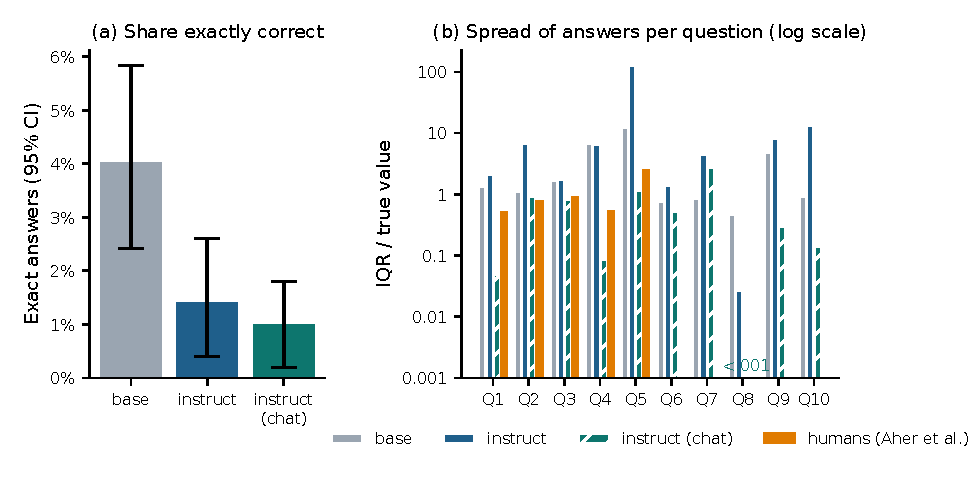
\includegraphics[width=\textwidth]{figures/fig_crowd_paper.pdf}
\caption{Own experiment. (a) Pooled share of exactly correct answers with 95\% bootstrap CI. (b) IQR divided by the true value per question (log scale); human values from Aher et al.~\cite{aher2023using}, Table~3, exist only for Q1--Q5. For Q8 (speed of light, true value 299,792,458) this ratio is tiny for every answer set and does not indicate accurate answers.}
\label{fig:crowd}
\end{figure}

\paragraph{Results.} Neither instruction-tuned condition shows the hyper-accuracy distortion (Table~\ref{tab:crowd}, Figure~\ref{fig:crowd}). No condition has an IQR of 0 on any question, and both instruct conditions give \emph{fewer} exact answers than the base model (\xInstExact{} and \xChatExact{} vs.\ \xBaseExact; Fisher \xInstFisherP{} and \xChatFisherP{}, both significant after correction). The spread depends on the prompt format: with the identical completion prompt, the instruct model spreads its answers \emph{more} widely than the base model on \the\numexpr10-\xInstLower\relax{} of 10 questions (Wilcoxon \xInstWilcP), whereas the chat format narrows the spread on \xChatLower{} of 10 questions (Wilcoxon \xChatWilcP); neither spread difference is significant after correction. In the chat format the median spread on Q1--Q5 (\xChatNIQRfive) is close to that of humans (\xHumNIQRfive), but the answers are centred on wrong values; for example, the median answer to ``How many bones does an adult human have?'' is 24. % SOURCE: research_poster/experiment/results/tables/per_question.csv (instruct_chat q01 median 24.0)
H1 is therefore not supported for this model size: instruction tuning alone did not produce exact, uniform answers. A plausible explanation, not tested here, is that the distortion needs both alignment and factual knowledge that a 0.5B model lacks; this fits Aher et al.'s observation that their smallest models did not show it either. % SOURCE: Aher et al. Table 3 p.25 (LM-1 to LM-3 medians far from truth, non-zero IQR)
The experiment is limited to one model size, one prompt wording and ten questions, and the human reference values are taken from the original study.
